\chapter{Intégration Continue}
\label{chap:integrationcontinue}

\section{Histoire}
La notion \textit{Intégration Continue} était mentionné dans un livre de Grady Booch en 1994 pour la première foi\footnote{\cite{boochooad}}. Il parlait d'une intégration continue par des publications interne et chaque publication apporte l'application plus proche à la version finale.

La prochaine foi que l'intégration continue était sous les feux de l'actualité était avec la publication des concepts de \textit{Extreme Programming} en forme d'un livre en 1999.
Là inclue est l'idée d'avoir une machine dédié à l'intégration du code et les pairs de développeurs réunissant, intégrant et testant le code source après chaque changement.\footnote{\cite{robertshistory}}

Une autre personne qui a gravé la notion \textit{Intégration Continue} est Martin Fowler. Il a publié un article sur le sujet en 2000 et révisé celui-ci six ans plus tard.\footnote{\cite{fowlerci}} Dans cet article il essayerait de donner une définition de l'IC et des meilleures pratiques. Martin Fowler travaillait chez ThoughtWorks, l'entreprise responsable pour la publication du première serveur d'\textit{Intégration Continue} "Cruise Control". Il est souvent cité comme personne-clé si on parle de l'IC.

Le premier livre publié sur la matière était "Continous Integration"\footnote{\cite{duvallconint}} en 2007. Naturellement il y a beaucoup d'autre livres traitant des technologie ou outils concrètes. Aujourd'hui le plus part d'entreprises implémentes quelques ou tous les aspects de l'IC.

\nocite{wikici}
\newpage

\section{Aperçu}
Pour pouvoir comprendre le concept de base de l'intégration continue il est nécessaire de connaitre le processus de développement logiciel ordinaire. L'intégration Continue n'exige pas de méthode de gestion de projets spécifique, mais est souvent utilisé avec des approches agiles, car elle les complètent parfaitement. Voici un diagramme d'un processus pareil. \footnote{Source http://www.techtipsnapps.com/2015/04/most-successful-software-development.html}

\begin{figure}[H]
	\centering
		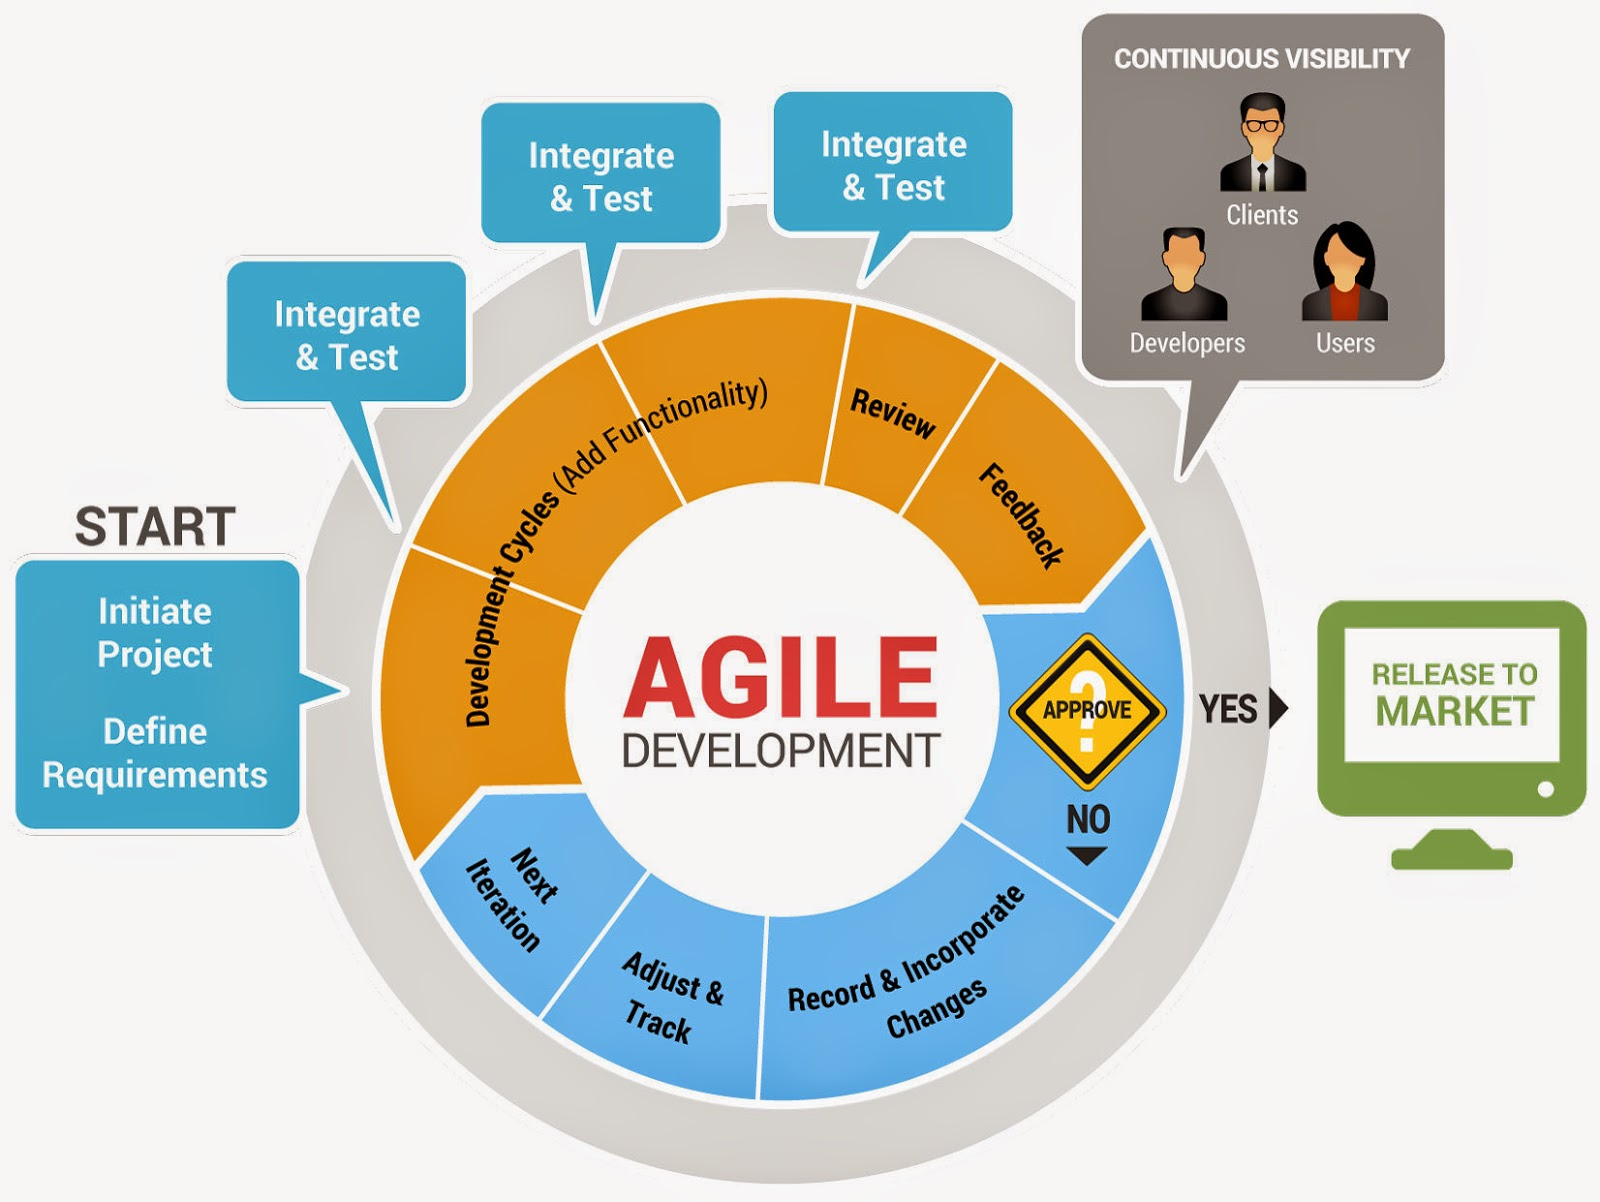
\includegraphics[scale=0.25]{bilder/agile_methodology}
	\caption{Processus de développement logiciel}
	\label{fig:processus}
\end{figure}

Les étapes récurrent sont le développement, les testes, les contrôles, le déploiement, la réaction du client et après ça une nouvelle itération. L'idée principale de L'IC est d'automatiser des devoirs des développeurs ou d'offrir des aides pendants tous ces étapes du processus de développement.
Pendant presque tous les projets de développement on travaille en équipe. Tous les développeurs font des changements et ajoutent de la fonctionnalité chaque jour. C'est pour cela qu'il est nécessaire de réunir ces changements régulièrement et de vérifier si tous les composants marche et coopère comme voulu (tests).\\\\
Ce processus de réunification s'appelle l'intégration. Si l'intégration est faite continuellement on parle de l'\textbf{Intégration Continue}. Mais une Intégration Continue à la lettre, chaque minute ou même en temps réel, n'est pas faisable ou aidant. C'est pour ça qu'une intégration exécuté au moins une foi par jour est normalement considéré suffisante, naturellement le plus souvent le mieux.\\
De plus cette intégration doit être facile et automatisée, comme pousser un bouton. Après lancer le processus d'intégration tous le reste doit être contrôlé par le système IC. La définition et l'étendue de l'IC est ouverte, pas strictement limité et fortement dépendant de l'application à développer. Mais il y a quelques éléments qui apparaissent dans tous les systèmes d'IC.
\newpage

\subsection{Architecture exemplaire}
Voici une architecture normale en travaillant avec un système d'intégration continue.
\begin{figure}[H]
	\centering
		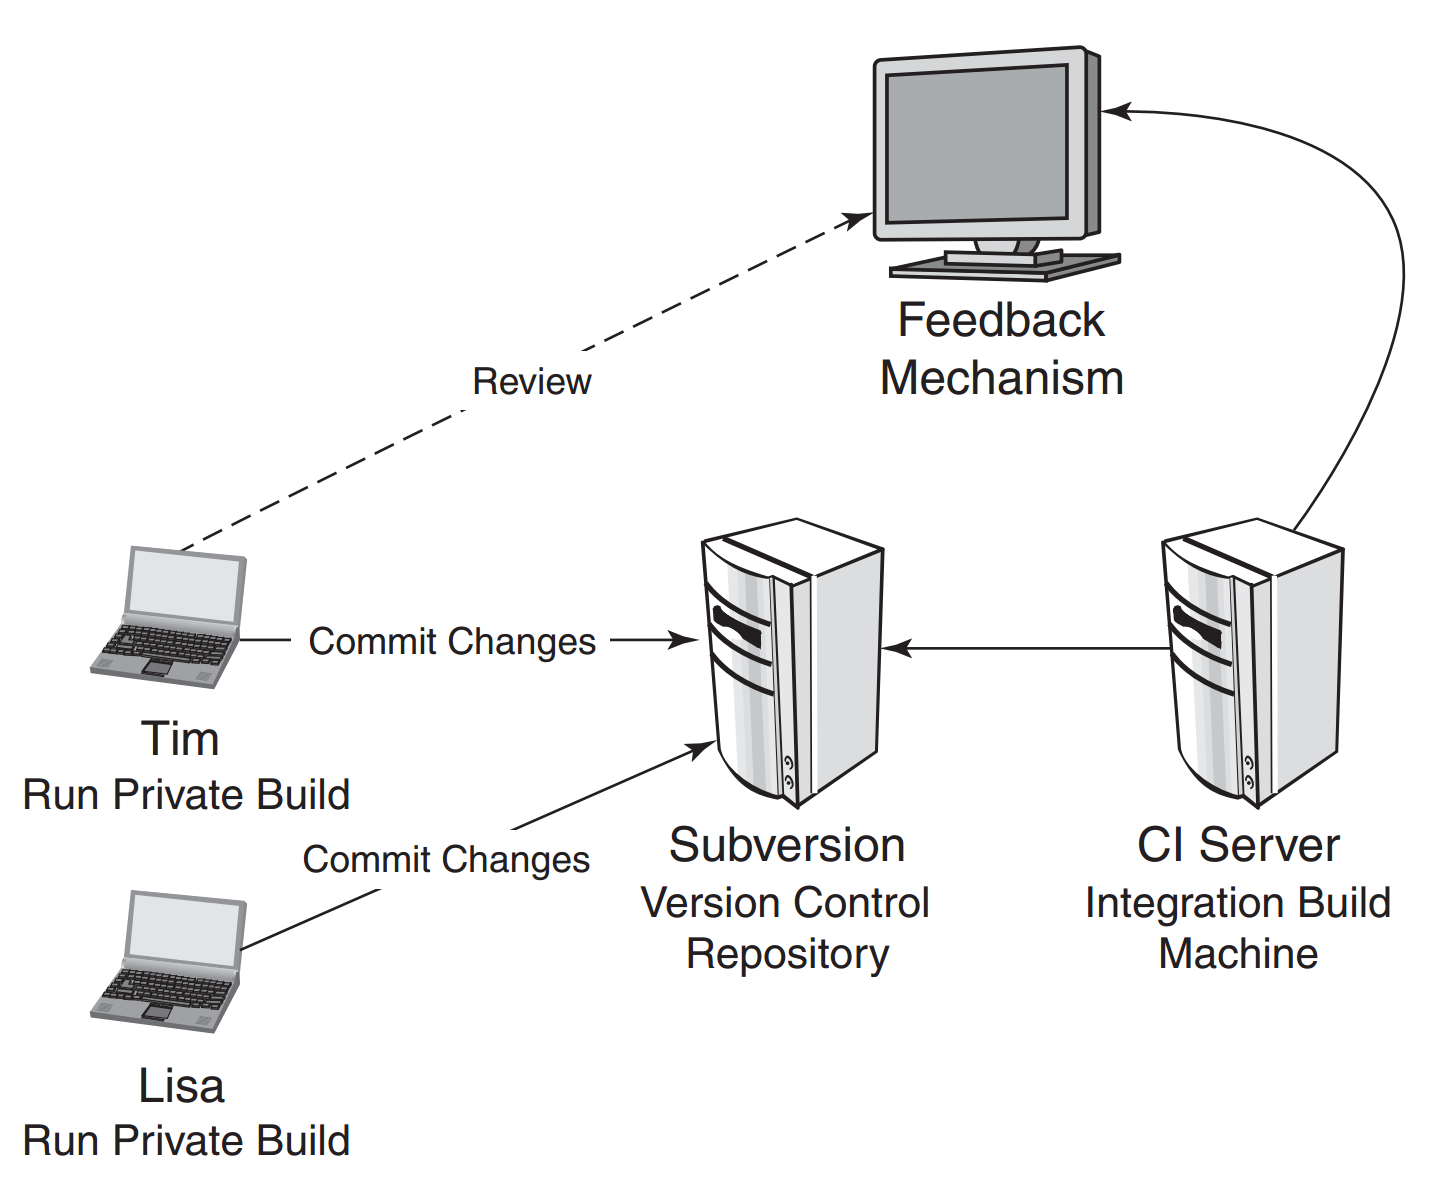
\includegraphics[scale=0.6]{bilder/architecture_exemplaire}
	\caption{Architecture exemplaire}
	\label{fig:processus}
\end{figure}

\textbf{Développement locale}\\
Tous les développeurs travaillent sur ses machines privées ou des machines de l'entreprise. Avant d'ajouter de la fonctionnalité la version la plus actuelle est téléchargé du dépôt centrale. Après changer le code il est nécessaire de faire une construction et d'exécuter les testes unitaires localement. Si tout fonctionne les changements sont commit sur le dépôt centrale.\\\\
\textbf{Dépôt centrale}\\
Le dépôt centrale est normalement un système de gestion de versions comme Subversion ou Git. Il est installé sur un serveur dédié. Tous les développeur reçoivent de l'accès pour commettre des changements là dessus. Ce faisant il est possible d'identifier qui a changé quoi en cas que quelque chose ne marche plus.\\\\
\textbf{Serveur de l'intégration continue} \\
Le serveur de l'intégration continue est la partie centrale du système. Il est aussi installé sur un serveur dédie, quelque foi sur la même machine que le dépôt centrale. Le serveur d'IC contrôle régulièrement s'il y a une nouvelle version dans le dépôt centrale. Si c'est le cas le serveur prends le code et démarre le processus d'intégration. Les étapes du processus doivent normalement être configurer une fois au début du projet. Quelques exemples pour des étapes possibles:
\begin{itemize}
\item Construction du code
\item Testes unitaires, testes d'intégration ou testes fonctionnelle
\item Inspections
\item Création de sous-système ou déploiement
\end{itemize}
Si on inclue le déploiement dans le processus d'intégration, il ne s'agit strictement plus seulement de l'intégration continue, mais aussi du \textbf{Déploiement et de la Livraison Continue} (Continous Deployment, Continuous Delivery). 
\\\\
\textbf{Information en retour}\\
Après finir ce processus d'intégration les résultats des étapes sont affiché sur un interface d'utilisateur centrale, souvent une page web. Pour toutes les étapes il est possible de configurer si l'échec de l'étape amène l'échec du processus complet. Si il y a des erreurs les développeurs et les personnes responsables peuvent être informé par des emails. Quelques entreprises installe des écrans dans les bureaux qui affichent les dernières résultats en temps réelle.\\
\section{Concepts de l'intégration continue}

\subsection{Construction continue}
L'idée de la construction continue est de définir le processus de construction une foi, normalement dans un fichier de construction, qui est ensuite utilisé par le serveur d'IC pour construire le projet à chaque intégration. Dans le fichier de construction les fichiers source et les dépendances sont définit. Tous les langages de programmation utilisent des outils de construction différents. Voici deux example.

\subsubsection{Java}
Ant (Another neat tool) est apparu en 2000, comme premier logiciel de construction pour Java.
Aujourd'hui Ant et ses produits de concurrence Maven(2002) et Gradle(2012) sont inévitable si on utilise Java.
Dans ce moment environ 70 \% des développeurs Java utilisent Maven, 15 \% Ant et 15\% Gradle. Le concept est pareille comme en C++. 
%EMAAA Quelle? VIDDY Ke ahnig me woni das uf em netz gfunde ha, weiss nur no das es veraltet isch gsi.. wahrschinlich isch gradle inzwüsche no höcher.. ha keni aktuelle statistike gfunde.. drum hani ja "environ" gschribe..
\subsubsection{C/C++}
Le premier logiciel de construction était make, qui existes depuis 1976 (Stuart Feldman, Bell Labs). Sur les plateformes basé sur Unix make est encore utilisé pour construire des exécutables.
Pour construire une application avec make if faut fournir un fichier makefile qui contiens les instructions de compilation. Supposant on a un logiciel avec les fichiers: \\ \\

\begin{tabular}{ll}
functions.h&squared.c\\
{\lstinputlisting[language=C]{../project/cpp_make_sample/functions.h}}&{\lstinputlisting[language=C,]{../project/cpp_make_sample/squared.c}}\\
\end{tabular}


factorial.c
\lstinputlisting[language=C]{../project/cpp_make_sample/factorial.c}


main.cpp
\lstinputlisting[language=C]{../project/cpp_make_sample/main.cpp}

La commande pour compiler ce projet manuellement est:
$$g++\;main.cpp\;squared.cpp\;factorial.cpp\;-o\;hello$$
Pour un projet si petit c'est assez simple, mais avec plus de fichiers ça devient continuellement plus difficile.
Par exemple si on a beaucoup de dépendances ou une application multi-plateforme, c'est très difficile de ne pas oublier un élément.
\newpage
C'est pour ça qu'il existe l'option de créer des makefile. Le makefile liste tous les fichiers et dépendances du projet.
\lstinputlisting[language=make,caption={Makefile sans variables}]{../project/cpp_make_sample/Makefile1.}
Si on regarde le fichier Makefile correspondant, on voit que ça ne simplifie pas encore notre vie. Une prochaine étape est l'introduction des variables dans le makefile.
\lstinputlisting[language=make,caption={Makefile avec variables}]{../project/cpp_make_sample/Makefile2.}

Ce fichier est plus court et très adaptable, mais il n'est pas vraiment lisible.
En utilisant l'outil cmake on peut générer les fichiers Makefile automatiquement (et autres fichiers de projet comme ".sln").
Dans le fichier CMakeLists.txt on définit quels fichiers il faut compiler et quels sont les dépendances.
\lstinputlisting[language=make,caption={CMakeLists.txt}]{../project/cpp_make_sample/CMakeLists.txt}

Tous ses types de construction peuvent être automatiser avec un serveur d'IC.
\newpage

\subsection{Intégration continue de base de données}

Le plus part de logiciel utilisent une méthode pour persister des données, beaucoup de fois des bases de données. Le code source pour générer cette base de données doit être traiter comme tous le reste du code d'un projet. C'est nécessaire qu'il soit aussi commit sur le dépôt centrale et qu'on teste et fait des inspections là dessus.

\subsubsection{Automatisation de l'intégration}
Si le code de la base de données est aussi mis sur le dépôt centrale, le processus de l'intégration de base de données peut être automatisé. Ce processus peut devenir assez complexe avec différent environnements. Les serveurs, les noms d'utilisateur, les mots de passe ou bien les données de test ou de système peuvent différer pour chaque environnement.
\begin{figure}[H]
	\centering
		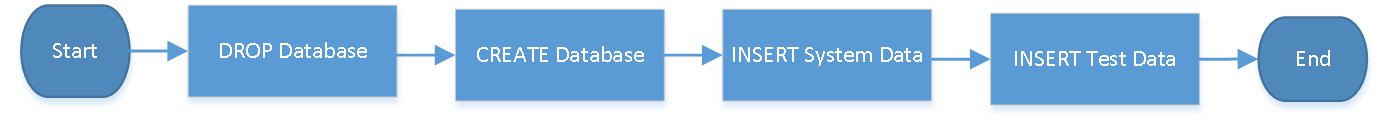
\includegraphics[scale=1]{bilder/database_integration}
	\caption{Processus de l'intégration de base de données}
	\label{fig:processus}
\end{figure}

C'est pour ça qu'une automatisation de ce processus est indispensable. Une automation est réalisé en insérant une section dans le script de construction uniquement pour les opérations de l'intégration de base de données. L'intervalle et l'étendue de l'exécution de ce processus sont pas les mêmes pour tous les projets. Pour quelques projets ça pourrait être trop lourds de recrée la base de données à chaque changement sur le dépôt centrale. Avec l'outil de construction Maven et le plugin "sql-maven-plugin" il est possible de définir quelle base de données est visé et quelles commandes sont exécuté. Voici une partie d'un tel script.\footnote{Pour l'exemple complète \cite{mvnsql}}

\lstinputlisting[language=XML]{./anhang/db_mvn_sql.xml}

\subsubsection{Instance de base de donnée locale}

Pour que cette approche fonctionne optimalement tous les développeurs doivent avoir l'autorisation de changer la définition de la base de données. Pour éviter des conflits pendant le développement tous les développeurs ont besoin d'une instance de cette base de données sur leur machines locales. Si on travaille avec une instance centrale à chaque changement il y a le danger de casser le code que quelqu'un d'autre est en train de développer.
\newpage


\subsection{Tests continue}
Les tests existes pour contrôler la fonctionnalité d'un bout de code, d'un système ou d'une application complète. Le premier principe de base pour des tests automatisés est "Fail fast" (Échouer vite). On distingue trois types de tests différents. Comme règle d'or on peut dire que les tests unitaires prend des secondes, les testes d'intégration prend des minutes et les tests d'acceptation prend des heures.\footnote{\citep{artofunittesting}}

\subsubsection{Tests unitaires}
Les tests unitaires vérifient le bon fonctionnement d'un bout de code. Pour les parties du code qui ne sont pas testable atomiquement on introduit des objets mock qui permettent des tests de fonctionnement vite et sans effets secondaires. 
\subsubsection{Tests d'intégration}
Après avoir testé les composant atomiquement, il est aussi nécessaire de tester l'interaction de ces composant avec des systèmes secondaire comme le système de fichier ou une base de données. Après ces tests d'intégration les erreurs logiques et d'intégration doivent être éliminé.
\subsubsection{Tests d'acceptation}
Les testes d'acceptation contrôle si les exigences du client sont respecté. \\
Il y a différents types de test d'acceptation:
\begin{enumerate}
 \item \textit{Tests d'interface utilisateur automatisé (code)}
 \\Pour ces tests il faut spécifier des scénario. Une programme teste accède l'application et exécute le scénario avec des interactions avec l'interface d'utilisateur.
 \item \textit{Tests de performance}
 \\Ces tests montrent quelles parties du code prennent la plupart des ressources et si le système est assez fort.
 \item \textit{Essais de pénétration}
 \\Si le logiciel utilise une base de données on peut par exemple tester la vulnérabilité contre des attaques injection SQL.
 \item \textit{Tests de charge}
 \\Par exemple: On a un magasin en ligne qui doit résister 100 utilisateurs à n'importe quel moment, testé avec les scénarios "login", "recherche des articles", "caisse", "login, ajouter, logout, login, effacer"
\end{enumerate}
\ \\
Le concept tests continue décrit le fait, que les tests doivent être exécuté régulièrement ou mêmes continuellement. Le serveur d'IC est configuré de lancer les tests après la construction quand il y a un changement sur le dépôt centrale. Car les trois différents types de tests ont une durée différente, on se restreinte normalement aux tests unitaires pour des constructions normale. Les testes d'intégration ou d'acceptation sont exécuté par le serveur d'IC pendant la nuit ou le weekend. C'est pour cela qu'il faut avoir multiple configuration de construction et de tests par projet.
\newpage

\subsection{Inspection continue}

La différence entre les tests et les inspections est que les inspections analyse la forme et la structure du code source et pas la fonctionnalité. Ces inspections sont introduit dans le processus de construction par différents plugins. Les inspections ne remplacent pas les contrôles code manuelles, mais dans ces contrôles il y aura moins de défauts banale à traiter. Les objectifs des inspections sont engrené là dessous.

\begin{enumerate}

\item \textit{Réduire la complexité du code source} \\ La complexité du code source peut être mesurée par la métrique "Cyclomatic Complexity Number (CCN)", qui compte le nombre de chemins distincts dans une méthode. Comme ça les endroits qui nécessite un changement peuvent être identifié (Plugin: JavaNCSS, PMD \footnote{\citep{pluginpmd}}).

\item \textit{Déterminer la dépendance} \\ Les métriques de couplage (Afferent/Efferent Coupling) et l'instabilité d'un paquet de logiciel peuvent être des indications à comme important un paquet est. Les paquets qui sont utilisé très souvent il vaut mieux les tester très exactement et être prudent avec des changements (Plugin: JDepend\footnote{\citep{pluginjdepend}}).

\item \textit{Imposer les standards de l'entreprise}\\ Dans chaque entreprise il y a des règles comment il faut écrire du code. Des exemples très fréquemment sont que les variables n'ose pas avoir des noms trop courts et non-descriptive ou que les déclarations conditionnel doivent toujours être écrit avec des parenthèses (Plugin: PMD).

\item \textit{Réduire le code copié} \\ Le code source copié doit être avouer. Il y a des outils qui identifie des sections de code identique (Plugin: PMD).

\item \textit{Déterminer la couverture de code} \\ La couverture de code par les testes est une métrique qui aide à déterminer quelles parties du code ont été négligé pendant écrire les testes (Plugin: Cobertura\footnote{\citep{plugincobertura}}).

\end{enumerate}

\begin{figure}[H]
\centering
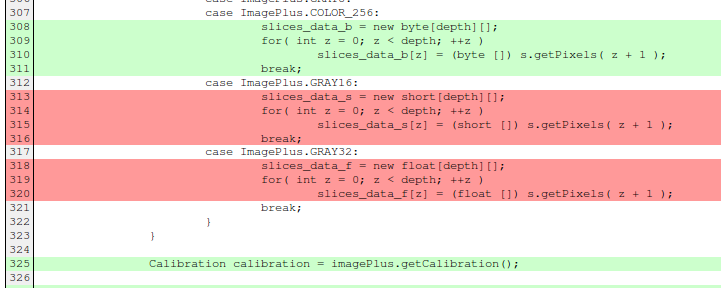
\includegraphics[width=15cm]{bilder/Coverage}
\caption{Couverture du code exemplaire} \cite{codecoverage}
\label{fig:coverage}
\end{figure}


\subsection{Information en retour continue}

Pendant le processus de construction, il est indispensable de savoir ce qui se passe. Chaque étape de construction doit fournir des informations à tous les personnes affecté. Classiquement c'est réalisé par envoyer un courriel aux personnes clés. Les possibilités plus modernes sont des plugins et notifications directement dans l'environnement de développement(Team Explorer for TFS intégré dans Visual Studio), dans une application de online-chat (TravisCI native, TeamCity, Jenkins avec plugins), comme message sur l'ordiphone ou dans le système d'exploitation (Native dans Windows 10 ou avec différents applications tierce partie).

\newpage
\subsection{Déploiement continue}

Le déploiement continue est un moyen pour délivrer la version actuelle d'une application aux utilisateurs immédiatement. Si un développeur fait un changement, la construction est initié automatiquement. Après ça les testes unitaires sont exécuté. Si tout les tests complète avec succès  le développeur est informé et l'exécution des testes d'acceptation automatisées commence. Si la fonctionnalité du logiciel est assuré une nouvelle version est déployé immédiatement.
Il est très probable que ce processus est différent pour chaque entreprise ou applications. Les testes d'utilisateur ou des autre contrôles manuelles pourrait être exiger.\\
\begin{figure}[H]
\centering
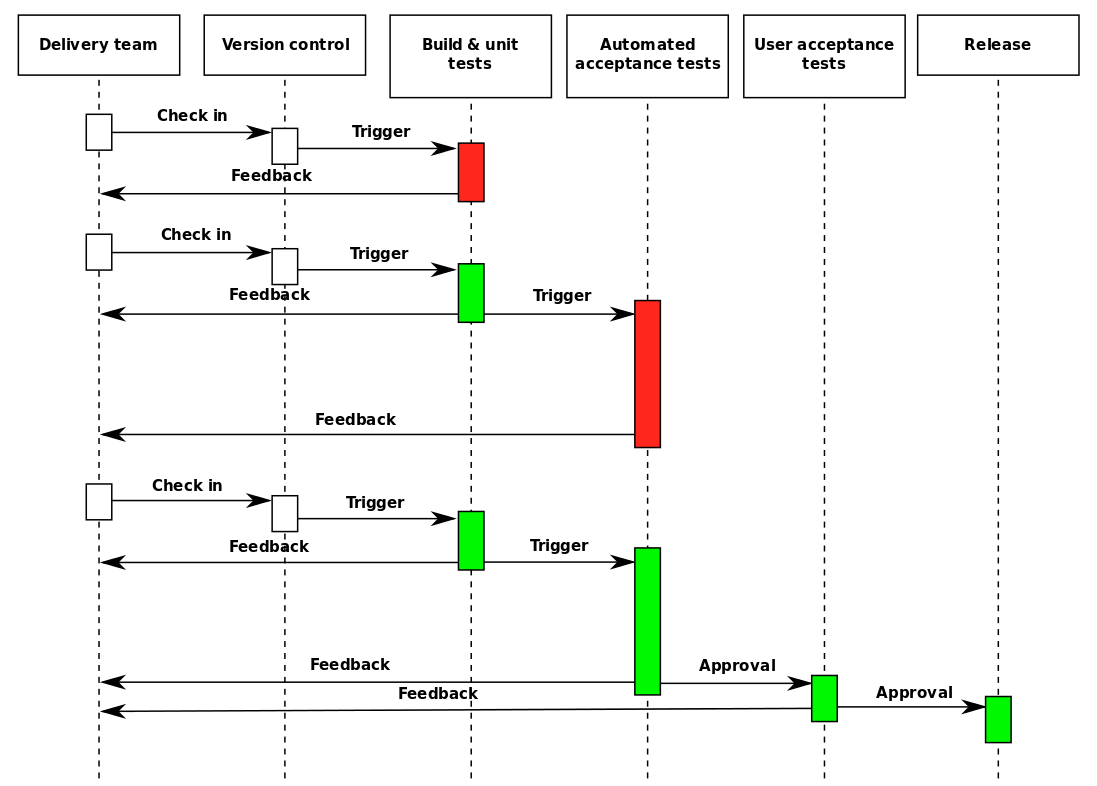
\includegraphics[width=15cm]{bilder/Continuous_Delivery}
\caption{Graphique déploiement continue}\cite{wikicd}
\label{fig:continousdelivery}
\end{figure}

Un autre scénario très fréquent est qu'on a plusieurs environnements et serveurs pour déployer une application (local, development, testing, production). Un déploiement sur la plateforme development seras moins critiques qu'un déploiement sur la production.

\begin{figure}[H]
\centering
\includegraphics[width=15cm]{bilder/Deployment_ci}
\caption{Déploiement continue - Environnements}\cite{bizagigraphique}
\label{fig:continousdelivery}
\end{figure}